\documentclass[titlepage]{article}
\usepackage[utf8]{inputenc}
\usepackage[czech]{babel}
\usepackage{graphicx}

\begin{document}
\begin{titlepage}
\begin{center}
	\mbox{} \\[3cm]
	\Huge{Semestrální práce z předmětu KIV/DB1} \\[.5cm]
	\huge{Půjčovna ponožek} \\[2.5cm]
	\Large{Tomáš Maršálek, A10B0632P} \\
	\large{marsalet@students.zcu.cz} \\[1cm]
	\normalsize{\today}
\end{center}
\thispagestyle{empty}
\end{titlepage}

\section{Popis úlohy}
Databáze slouží hypotetické půjčovně ponožek především k uchovávání údajů realizovaných vypůjčení, přehledu zákazníků, zboží a personálu.

\section{Datový model}
Databáze se skládá z šesti tabulek, kde jedna tabulka představuje číselník.
Každá z tabulek obsahuje sloupec id, který ve všech tabulkách představuje
primární klíč a databáze podle něj vytvoří index.

\begin{figure}
\centering
	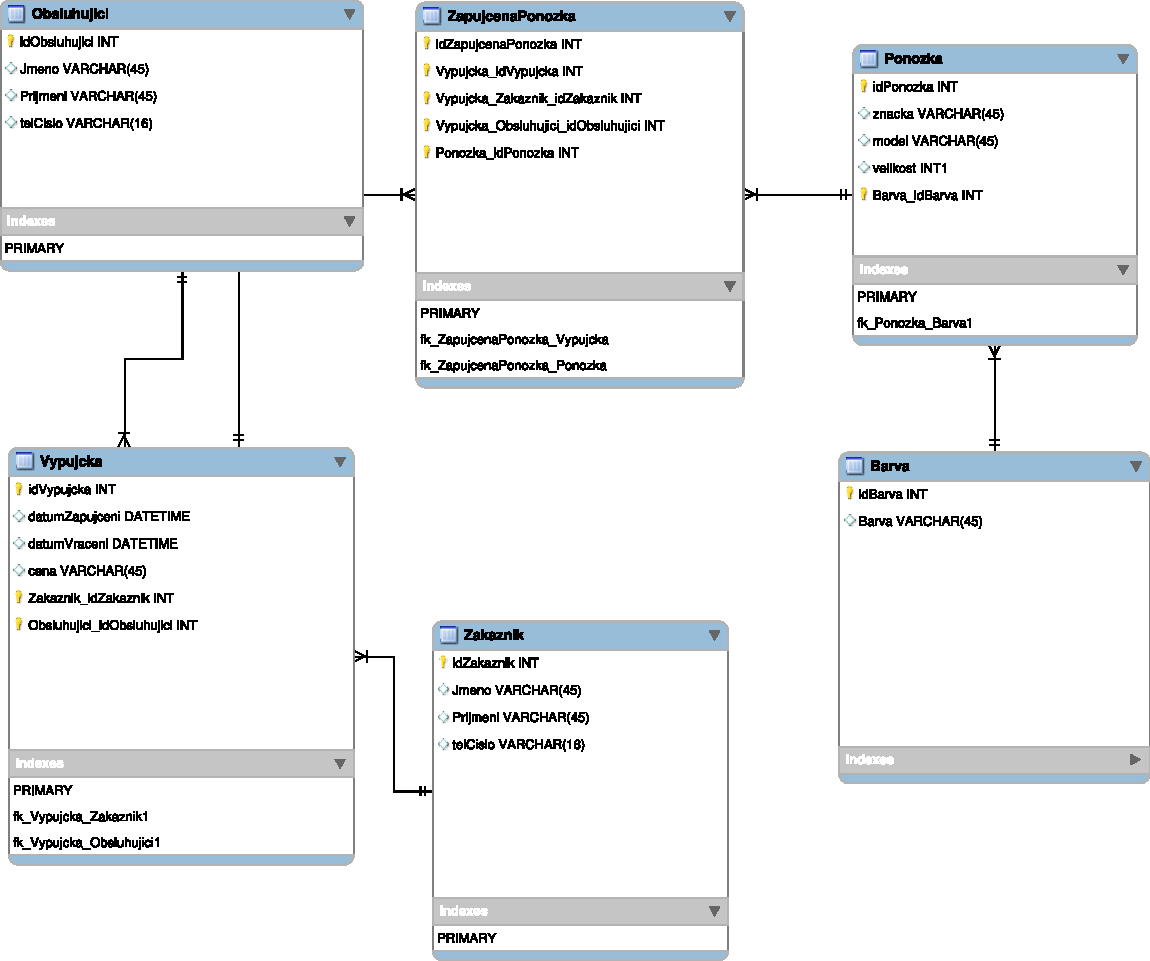
\includegraphics[width=\textwidth,angle=90]{eer.pdf}
	\caption{EER model}
\end{figure}

\subsection{Zákazník}
Půjčovna ani v praktickém použití nepotřebuje o zákazníkovi vědět přespříliš
údajů. Navíc by bylo nepříjemné při obyčejném vypůjčení jakéhokoliv zboží
vyplňovat všelijaké otravné formuláře a dotazníky. Po zákazníkovi pouze chceme
Jméno, Příjmení a jako kontaktní informaci telefonní číslo.

\subsection{Obsluhující}
Stejně jako v případě zákazníka příliš nesledujeme osobní údaje personálu
půjčovny, pouze Jméno, Příjmení a opět telefonní číslo. Samozřejmě zde by bylo
možné přidat údaje pro zaslání výplaty, tedy bankovní účet nebo adresu
bydliště. Nicméně pro ukázkové účely této databáze stačí pouze pár údajů.

\subsection{Ponožka}
Celá půjčovna se prakticky točí kolém této tabulky, bez ní by ani neměla smysl.
I když je v názvu ponožka v jednotném čísle, samozřejmě se jedná o pár.
Nezbytné údaje pro třídění ponožek jsou v tomto případě značka (výrobce), model
neboli jakési pojmenování typu ponožky od výrobce, barva a velikost v míře
kontinentální evropy pro velikosti bot. Barva není typu řetězce, ale je pouze
cizím klíčem na číselník Barva.

\subsection{Barva}
Barva je pouze číselník, který slouží k dekompozici schématu. Obsahuje své id a
řetězec s názvem barvy.

\subsection{Výpůjčka}
Tato tabulka je klíčovou tabulkou při uchovávání údajů o vypůjčení a v datovém
modelu spojuje tabulky, které slouží k uchovávání konečných dat (Ponožka,
Obsluhující, Zákazník). Mimo svůj primární klíč id obsahuje cizí klíče
zákazníka a obsluhujícího.  V praktickém použití tedy říká, který zákazník
provedl vypůjčení u kterého konkrétního člena personálu. Mimo cizí klíče ještě
obsahuje datum zapůjčení a vrácení a cenu. Cena zde není nikterak vypočítávána
na základě doby vypůjčení, počtu ponožek nebo typu ponožek. Tato funkcionalita
by byla v praktické databázi vyžadována.

\subsection{Zapůjčená ponožka}
Poslední tabulka je produktem rozkladu schématu mezi tabulkami Ponožka a
Výpůjčka. Mezi nimi je totiž relace typu $N$ ku $N$, kterou rozložíme na další
tabulku (tuhle), spojenou s původními dvěma tabulkami relací $1$ ku $N$.
Tabulka Výpůjčka má přehled pouze o zákazníkovi a obsluhujícím, kteří se
podíleli na vypůjčení. Tahle tabulka jí přidává poslední potřebný údaj, a to
které konkrétní ponožky vlastně byly zapůjčeny. V tabulce Výpůjčka bychom
tenhle údaj nemohli zaznamenat, protože se jedná o seznam ponožek, ne jen o
jednu ponožku. Tedy tabulka má sloupce své id, cizí klíče ponožky a výpůjčky,
žádné další informace neobsahuje.

\section{Dotazy}
\subsection{Zákazníci milující hnědé ponožky}
Výsledkem prvního z dotazů je seznam všech zákazníků, kteří jsou evidováni, že
si někdy vypůjčili pár ponožek hnědé barvy. Dotaz spojuje všechny tabulky
databáze mimo tabulky obsluhujícího do jedné pomocí $INNER JOIN$u a filtruje na
základě barvy ponožek.
\begin{verbatim}
SELECT 
	Prijmeni, 
	Jmeno, 
	Znacka, 
	Model, 
	Barva
FROM 
	Zakaznik
	INNER JOIN Vypujcka
	ON idZakaznik = Zakaznik_idZakaznik
	INNER JOIN ZapujcenaPonozka
	ON idVypujcka = Vypujcka_idVypujcka
	INNER JOIN Ponozka
	ON idPonozka = Ponozka_idPonozka
	INNER JOIN Barva
	ON idBarva = Barva_idBarva
WHERE 
	Barva =  'hnědá'
ORDER BY
	Prijmeni ;
\end{verbatim}

\subsection{Zákazníci a obsluhující, kteří se nevidí poprvé}
Další dotaz demonstruje využití agregačních funkcí jazyka SQL v příkladě, kdy
hledáme všechny zákazníky a obsluhující, u nichž existuje více než jedna
výpůjčka, na níž se podíleli konkrétní zákazník a obsluhující. Zkrátka, pokud
přišel zákazník podruhé a byl obsloužen stejným člověkem jako minule, bude
obsažen ve výsledku tohoto dotazu.
\begin{verbatim}
SELECT 
	Zakaznik.Jmeno, 
	Zakaznik.Prijmeni, 
	COUNT(*) AS c, 
	Obsluhujici.Jmeno, 
	Obsluhujici.Prijmeni 
FROM 
	Zakaznik 
	INNER JOIN Vypujcka 
	ON idZakaznik = Zakaznik_idZakaznik 
	INNER JOIN Obsluhujici 
	ON idObsluhujici = Obsluhujici_idObsluhujici 
GROUP BY idZakaznik 
HAVING c > 1
ORDER BY c DESC ;
\end{verbatim}

\section{Implementace}
Pro práci bylo zvoleno prostředí MySql. ERR model byl vytvořen v aplikaci {\bf
mysql-workbench}. Databázové schéma bylo na lokálním serveru vytvořeno v téže
aplikaci a data vložena pomocí {\bf phpmyadmin}, ale pro zrekonstruování
vložení dat do prázdné databáze byl vytvořen ekvivalentní sql skript.

\section{Závěr}
Databázi by bylo možné použít v existující půjčovně ponožek, pokud nějaká
existuje. Bylo by ale vhodné doplnit několik sloupců do patřičných tabulek, aby
dostačovala pro reálné použití.

\end{document}
